\documentclass[a4paper,11pt]{article}
\usepackage[utf8]{inputenc}
\usepackage{amsmath}
\usepackage{amsfonts}
\usepackage{amssymb}
\usepackage{graphicx}
\usepackage{braket}

\numberwithin{equation}{section}
\renewcommand\thesubsection{\alph{subsection}}
\newcommand{\bvp}[1]{\mathbf{#1}'}
\newcommand{\bv}[1]{\mathbf{#1}}
\newcommand{\ez}{\epsilon_0}
\newcommand{\lrp}[1]{\left({#1}\right)}
\newcommand{\lrb}[1]{\left\{{#1}\right\}}


%opening
\title{Electromagnetic Theory I HW3}
\author{Vince Baker}

\begin{document}

\maketitle

\section{Problem 2.1}
a) Using the method of images, the image of charge $q$ at distance $z=d$ from an infinite conductor on the $x-y$ plane is a charge $-q$ at $z=-d$.
We first solve for the potential, which is simply the sum of the potential from the actual and image charges.
\begin{align}
 \Phi(x,y,z\ge 0) &= \frac{q}{4\pi\ez}\lrp{\frac{1}{\lrp{x^2+y^2+(z-d)^2}^{1/2}}}-\frac{q}{4\pi\ez}\lrp{\frac{1}{\lrp{x^2+y^2+(z+d)^2}^{1/2}}}
\end{align}
To find the surface charge density, we use:
\begin{align}
 \sigma &= -\ez\frac{\partial \Phi}{\partial z}|_{z=0}\\
 \sigma &= -\frac{q}{4\pi}\lrb{\frac{-z+d}{\lrp{x^2+y^2+(z-d)^2}^{3/2}}+\frac{z+d}{\lrp{x^2+y^2+(z+d)^2}^{3/2}}}\\
 \sigma &= -\frac{q}{2\pi}\frac{d}{\lrp{x^2+y^2+d^2}^{3/2}}
\end{align}
b) The Coulomb's law force between the particles is:
\begin{align}
 F &= -\frac{1}{4\pi\ez}\frac{q^2}{4d^2}\hat{z}\\
 F &= -\frac{1}{16\pi\ez}\frac{q^2}{d^2}\hat{z}
\end{align}
c) Calculating the force as the integral of $\sigma^2$ over the plane:
\begin{align}
 \sigma^2 &= \frac{1}{4\pi^2}\frac{q^2d^2}{\lrp{x^2+y^2+d^2}^3}
\end{align}
Integrating over the plane in polar coordinates:
\begin{align}
 F &= \int_0^{2\pi}\int_0^\infty \frac{\sigma^2}{2\ez} r\ dr d\theta\\
 F &= \frac{q^2d^2}{4\pi\ez}\int_0^\infty \frac{r}{\lrp{r^2+d^2}^3} dr\\
 F &= \frac{1}{16\pi\ez}\frac{q^2}{d^2}
\end{align}
So the force on the image particle and the total force on the plane are the same, as expected.
\\
d) We integrate the force on the particle as we move the particle from d to $\infty$.
\begin{align}
 W &= \int F\cdot d\ell = \frac{q^2}{16\pi\ez}\int_d^\infty \frac{1}{d^2} d\ell\\
 W &= \frac{1}{16\pi\ez}\frac{q^2}{d}
\end{align}
e) For two charges of magnitude $q$ and $-q$ separated by distance $2d$, the potential energy is:
\begin{align}
 PE &= -\frac{q^2}{8\pi\ez d}
\end{align}
This is twice the potential energy of the single charge found in part d.
We are counting the image charge as a separate charge, but in fact the image charge only exists due to the influece of the actual charge.
Part d is the correct calculation of the potential energy, since it correctly calculates the field from the image charge along the path of integration of the real charge.
\\
f) For an elementary charge one angstrom from the surface, the result from part d gives $5.767e^{-19}$ Joules, or 3.6 electron-volts.


\section{Problem 2.3}
a) We solve the problem using the method of images.
It is clear that the image line charge for the $x=0$ plane (call it A) should have charge density $-\lambda$ and be placed at $(-x_0,y_0)$.
The image line charge for the $y=0$ plane (call it B) should have charge density $-\lambda$ and be placed at $(x_0,-y_0)$.
We are now left with the residual potential of line charge A on the plane at $y=0$ and of line charge B on the plane at $x=0$.
However, we see that placing an additional line charge of density $+\lambda$ at $(-x_0,-y_0)$ (call it C) will cancel the residual contributions from both A and B.
\\
We now have the expression for the potential of this configuration:
\begin{align}
 \begin{split}
 \frac{4\pi\ez}{\lambda}\Phi(x,y) = &\ln{\lrp{\frac{R^2}{(x-x_0)^2+(y-y_0)^2}}}
	      -\ln{\lrp{\frac{R^2}{(x+x_0)^2+(y-y_0)^2}}}\\
	      &-\ln{\lrp{\frac{R^2}{(x-x_0)^2+(y+y_0)^2}}}
	      +\ln{\lrp{\frac{R^2}{(x+x_0)^2+(y+y_0)^2}}}
 \end{split}
\end{align}
Inserting $x=0$ and $y=0$ we see that the potential is zero on the boundary surfaces as expected.
To check the tangential electric field we take the partial derivatives with respect to x and y:
\begin{align}
 \begin{split}
 \frac{4\pi\ez}{\lambda}\frac{\partial \Phi}{\partial x} = &-2\frac{x-x_0}{(x-x_0)^2+(y-y_0)^2}
      +2\frac{x+x_0}{(x+x_0)^2+(y-y_0)^2}\\
      &+2\frac{x-x_0}{(x-x_0)^2+(y+y_0)^2}
      -2\frac{x+x_0}{(x+x_0)^2+(y+y_0)^2}
 \end{split}\\
 \begin{split}
 \frac{4\pi\ez}{\lambda}\frac{\partial \Phi}{\partial y} = &-2\frac{y-y_0}{(x-x_0)^2+(y-y_0)^2}
      +2\frac{y-y_0}{(x+x_0)^2+(y-y_0)^2}\\
      &+2\frac{y+y_0}{(x-x_0)^2+(y+y_0)^2}
      -2\frac{y+y_0}{(x+x_0)^2+(y+y_0)^2}
 \end{split}
\end{align}
The first expression is the tangential electric field along the $y=0$ plane. 
Plugging in $y=0$ we see that the terms cancel and therefore the tangential electric field is 0 as expected.
The second expression is the tangential electric field along the $x=0$ plane. 
Plugging in $x=0$ we see that the terms cancel and therefore the tangential electric field is 0 as expected.
\\
b) The surface charge density is related to the discontinuity of the electric field across the surface:
\begin{align}
 \Delta E &= \frac{\sigma}{\ez}
\end{align}
Assuming there is no (actual) charge other than the line charge in the first quadrant, the electric field on the other side of the conducting planes is zero.
Therefore, with the normal to the surface pointing in the $-y$ direction, the the surface charge density on the $y=0$ plane is:
\begin{align}
 \sigma &= -\ez E_y
\end{align}
Plugging $y=0$ into equation 3 we find:
\begin{align}
 \begin{split}
 \frac{4\pi\ez}{\lambda}\frac{\partial \Phi}{\partial y} = &2\frac{y_0}{(x-x_0)^2+y_0^2}
      -2\frac{y_0}{(x+x_0)^2+y_0^2}\\
      &+2\frac{y_0}{(x-x_0)^2+y_0^2}
      -2\frac{y_0}{(x+x_0)^2+y_0^2}
 \end{split}\\
 E_y &= \frac{\lambda}{\pi\ez}\lrb{\frac{y_0}{(x-x_0)^2+y_0^2}-\frac{y_0}{(x+x_0)^2+y_0^2}}\\
 \sigma &= -\frac{\lambda}{\pi}\lrb{\frac{y_0}{(x-x_0)^2+y_0^2}-\frac{y_0}{(x+x_0)^2+y_0^2}}
\end{align}
The surface charge densities are plotted below.\\
\begin{figure}[h]
 \caption{Surface charge density along y=0 plane}
 \centering
   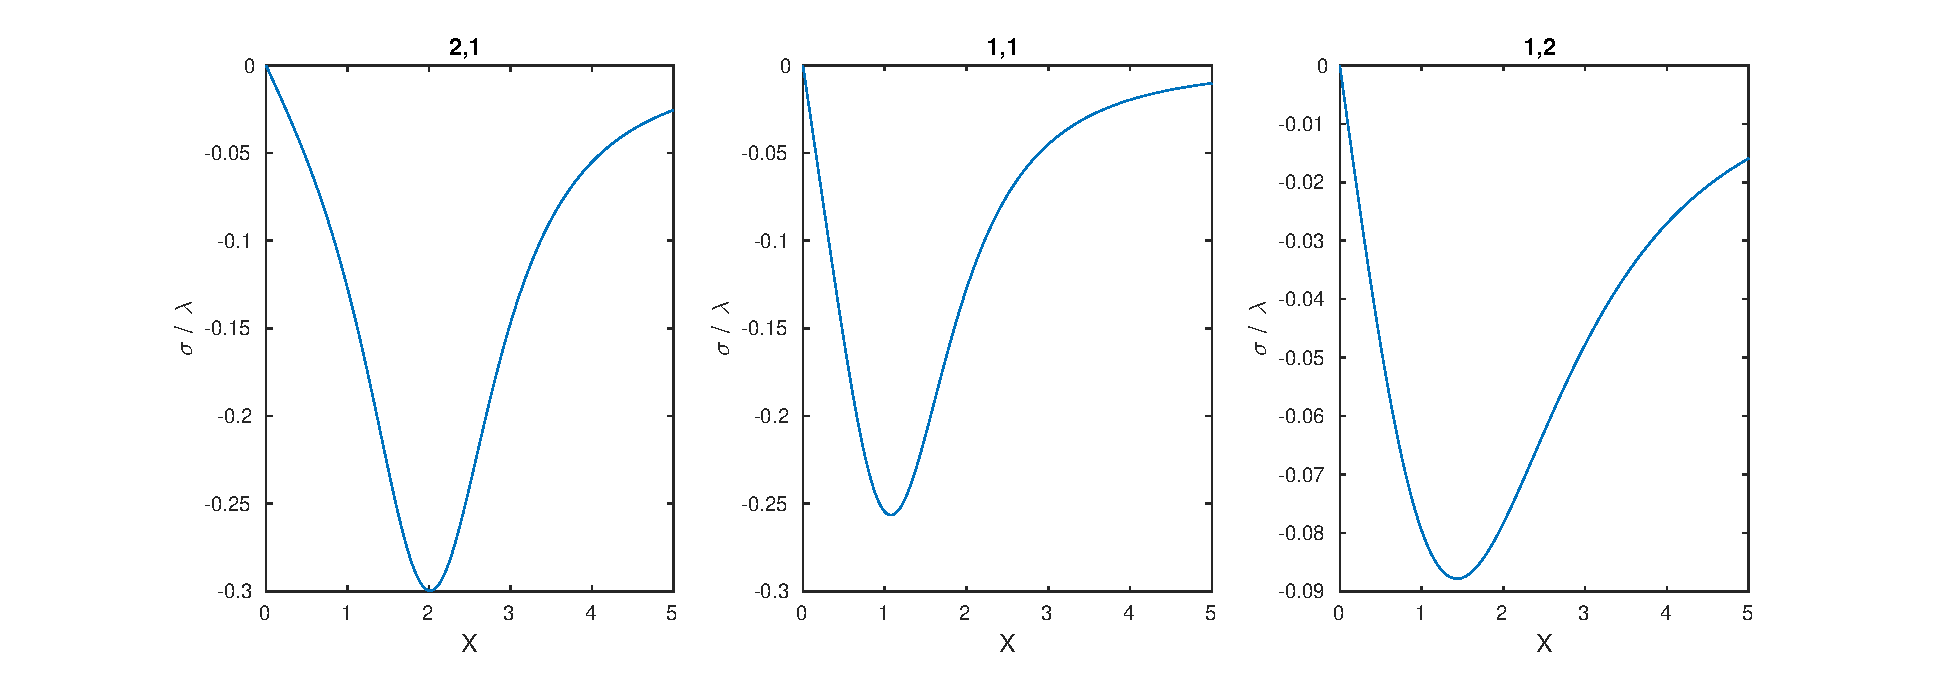
\includegraphics[width=\textwidth]{p2_3}
\end{figure}

\section{Problem 2.7abc}
a) We are looking for the apropriate Green's function such that $G(x,x^\prime)$ vanishes on the boundary surface.
We have already found, using the method of images, a potential function that vanishes on a planar boundary surface.
Using the method of images result, we find:
\begin{align}
 \begin{split}
 G(x,x^\prime) = &\frac{1}{\lrp{(x-x')^2+(y-y')^2+(z-z')^2}^{1/2}}\\
		 &-\frac{1}{\lrp{(x-x')^2+(y-y')^2+(z+z')^2}^{1/2}}
 \end{split}
\end{align}
b) With Dirichlet boundary conditions, the potential is:
\begin{align}
 \Phi(x,x') &= \frac{1}{4\pi\ez}\int_v\rho(x')G(x,x')d^3x'-\frac{1}{4\pi}\oint_S\Phi(x')\frac{\partial G(x,x')}{\partial n}da'
\end{align}
We are given the potential on the plane but no charge distribution, so we assume the first term is zero.
The boundary surface extends to inifinity, so we only expect a contribution to the integral from the disc of potential V on the plane.
Writing the integral in cylindrical coordinates, using our results from problem 2.3 for the derivative in the z direction at $z'=0$,
and recognizing that the normal points in the $-z$ direction:
\begin{align}
 \Phi(r,\theta,z) &= \frac{V}{4\pi}\int_0^a\int_0^{2\pi}\lrp{\frac{2z}{\lrp{(x-x')^2+(y-y')^2+z^2}^{3/2}}}r'\ dr'd\theta'\\
 \Phi(r,\theta,z) &= \frac{Vz}{2\pi}\int_0^a\int_0^{2\pi}\lrp{\frac{r'}{\lrp{r^2+{r'}^2-2r{r'}\cos{(\theta-\theta')}+z^2}^{3/2}}}\ dr'd\theta'
\end{align}
c) Along the axis of the disc $(r=0)$ we can solve the integral to find the potential.
\begin{align}
 \Phi(0,\theta,z) &= \frac{Vz}{2\pi}\int_0^a\int_0^{2\pi}\lrp{\frac{r'}{\lrp{{r'}^2+z^2}^{3/2}}}\ dr'd\theta'\\
 \Phi(0,\theta,z) &= Vz\int_0^a\lrp{\frac{r'}{\lrp{{r'}^2+z^2}^{3/2}}}\ dr'\\
 \Phi(0,\theta,z) &= Vz\lrb{-\frac{1}{\sqrt{{r'}^2+z^2}}}_0^a\\
 \Phi(0,\theta,z) &= V\lrp{1-\frac{z}{\sqrt{a^2+z^2}}}
\end{align}



\end{document}
